\documentclass{beamer}
\usetheme{JuanLesPins}

\usepackage{fontspec}
\usepackage[catalan]{babel}
\usepackage{verbatim}
\usepackage{listings}
\usepackage{upquote}
\usepackage{color}
\definecolor{bluekeywords}{rgb}{0.13,0.13,1}
\definecolor{greencomments}{rgb}{0,0.5,0}
\definecolor{redstrings}{rgb}{0.9,0,0}
\lstdefinelanguage{FORTH}
{   
    morekeywords={+, *, -, DO, LOOP, EMIT, DUP, DROP, CR, CHAR },
    keywordstyle=\color{bluekeywords},
    sensitive=false,
    basicstyle=\ttfamily,
    breaklines=true,
    xleftmargin=\parindent,
    aboveskip=\bigskipamount,
    tabsize=4,
    morecomment=[l][\color{greencomments}]{\\},
    morecomment=[s][\color{greencomments}]{( }{--\ )},
    morestring=[b]",
    showstringspaces=false,
    literate={}{\ }1,
        stringstyle=\color{redstrings},
}
\lstset{language=FORTH} 


\title{FORTH}
\subtitle{Llenguatges de Programació}
\author{Joan Marcè i Igual}
\institute[UPC]{Universitat Politècnica de Catalunya}
\date{Maig 2016}

\AtBeginSection[]
{
    \begin{frame}
        \frametitle{Contingut}
        \tableofcontents[currentsection,currentsubsection]
    \end{frame}
}

\AtBeginSubsection[]
{
    \begin{frame}
        \frametitle{Contingut}
        \tableofcontents[currentsection,currentsubsection]
    \end{frame}
}

\begin{document}

\frame{\titlepage}

\section{Introducció}

\begin{frame}
    \begin{columns}[c]
        \begin{column}{0.5\linewidth}
            FORTH va ser dissenyat per \emph{Charles Chuck Moore}. Va ser creat als voltants de 1968 orientat a la indústria aeroespacial. \\
            \pause
            El nom fa referència a que havia de ser la quarta generació de llenguatges
            (ve de \emph{fourth} en anglès però la \emph{u} no es va posar perquè el SO utilitzat només suportava 5 caràcters per als noms d'arxius).
        \end{column}
        \begin{column}{0.5\linewidth}
            \onslide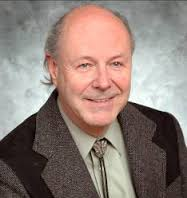
\includegraphics[height=0.5\textheight]{charles}    
        \end{column}

    \end{columns}
\end{frame}

\begin{frame}
    \frametitle{Influències}
    \begin{columns}[c]
        \begin{column}{0.7\linewidth}
            El llenguatge va ser influenciat per:
            \begin{itemize}
                \item Burroughs large systems
                \item Lisp
                \item APL
            \end{itemize}
        \end{column}
        \begin{column}{0.3\linewidth}
            \centering
            
\includegraphics[width=.8\linewidth]{lisplogo}\\
            
\includegraphics[width=.8\linewidth]{apllogo}
        \end{column}
    \end{columns}
\end{frame}

\section{Principals característiques}
\subsection{Paradigma}
\begin{frame}[fragile]
    
    FORTH és un llenguatge imperatiu i que funciona amb un sistema de pila.
    
    \begin{lstlisting}[frame=single]
    \Exemple per realitzar (25 * 10) + 50
    25 10 * 50 +
    \end{lstlisting}
    \begin{lstlisting}[frame=single,language=TeX]
    300 ok
    \end{lstlisting}
\end{frame}

\subsection{Compilat o interpretat?}
\begin{frame}
    FORTH és un llenguatge pensat perquè sigui interpretat mitjançant comandes però també es poden compilar diverses seqüències de comandes per a ser utilitzades més tard.
    \vfill
    \centering
    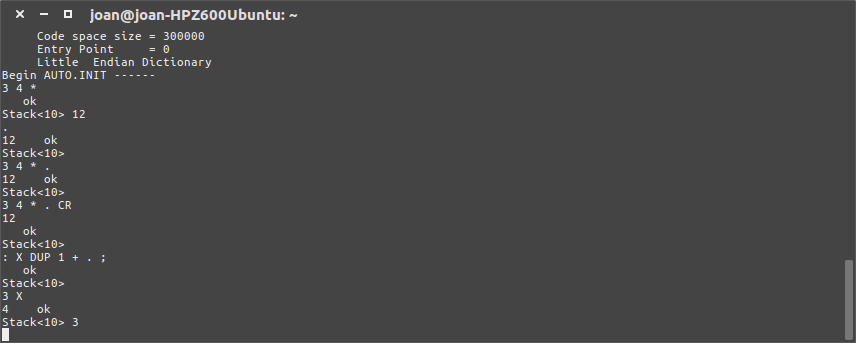
\includegraphics[height=0.5\textheight]{console_1}
\end{frame}

\subsection{Sistema de tipus}

\begin{frame}
    En FORTH hi ha diferents tipus però no es fa comprovació de tipus, és a dir, si el programador s'equivoca al cridar una funció (per exemple es passa un float en lloc d'un enter) les dades seran interpretades erròniament.
    
    A més a més, no hi ha sobrecàrrega d'operadors pel que totes les funcions han de tenir noms diferents.
    Per exemple per sumar existeixen les següents operacions
    \texttt{+, f+, c+, u+}
\end{frame}

\subsection{Sistema de pila}

\begin{frame}[fragile]
    FORTH utilitza una pila per implementar totes les seves operacions
    
    \begin{lstlisting}[frame=single]
    \Exemple per realitzar (25 * 10) + 50
    25 10 * 50 +
    \end{lstlisting}
    
    \centering
    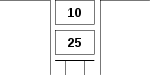
\includegraphics[width=0.2\linewidth]{stack_1}
    \hfill
    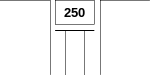
\includegraphics[width=0.2\linewidth]{stack_2}
    \hfill
    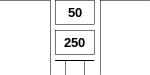
\includegraphics[width=0.2\linewidth]{stack_3}
    \hfill
    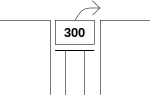
\includegraphics[width=0.2\linewidth]{stack_4}
\end{frame}

\section{Exemples}

\begin{frame}[fragile]
    
    \begin{lstlisting}[frame=single, basicstyle=\tiny\ttfamily]
: STAR ( -- )           \Imprimeix * per pantalla          
  [CHAR] * EMIT ;       \ $ STAR
                        \ *

: STARS     ( n -- )    \Imprimeix n estrelles
  0 DO STAR LOOP        \Fer n iteracions (de 0 a n-1) i executa
  STAR ;                \ $ 3 STARS
                        \ ***
  
: SQUARE    ( n -- )    \Imprimir n^2 estrelles en forma de quadrat
  DUP 0 DO              \ $ 3 SQUARE
  DUP STARS CR          \ ***
  LOOP DROP ;           \ ***
                        \ ***
  
: TRIANGLE  ( n -- )    \Imprimir un triangle de n-línies
  1 + 1 DO              \ $ 3 TRIANGLE
  I STARS CR            \ *
  LOOP ;                \ **
                        \ ***
    \end{lstlisting}
\end{frame}

\begin{frame}
    \frametitle{Llenguatges similars}
    Com a llenguatges similars hi ha el RPL de les calculadores HP
    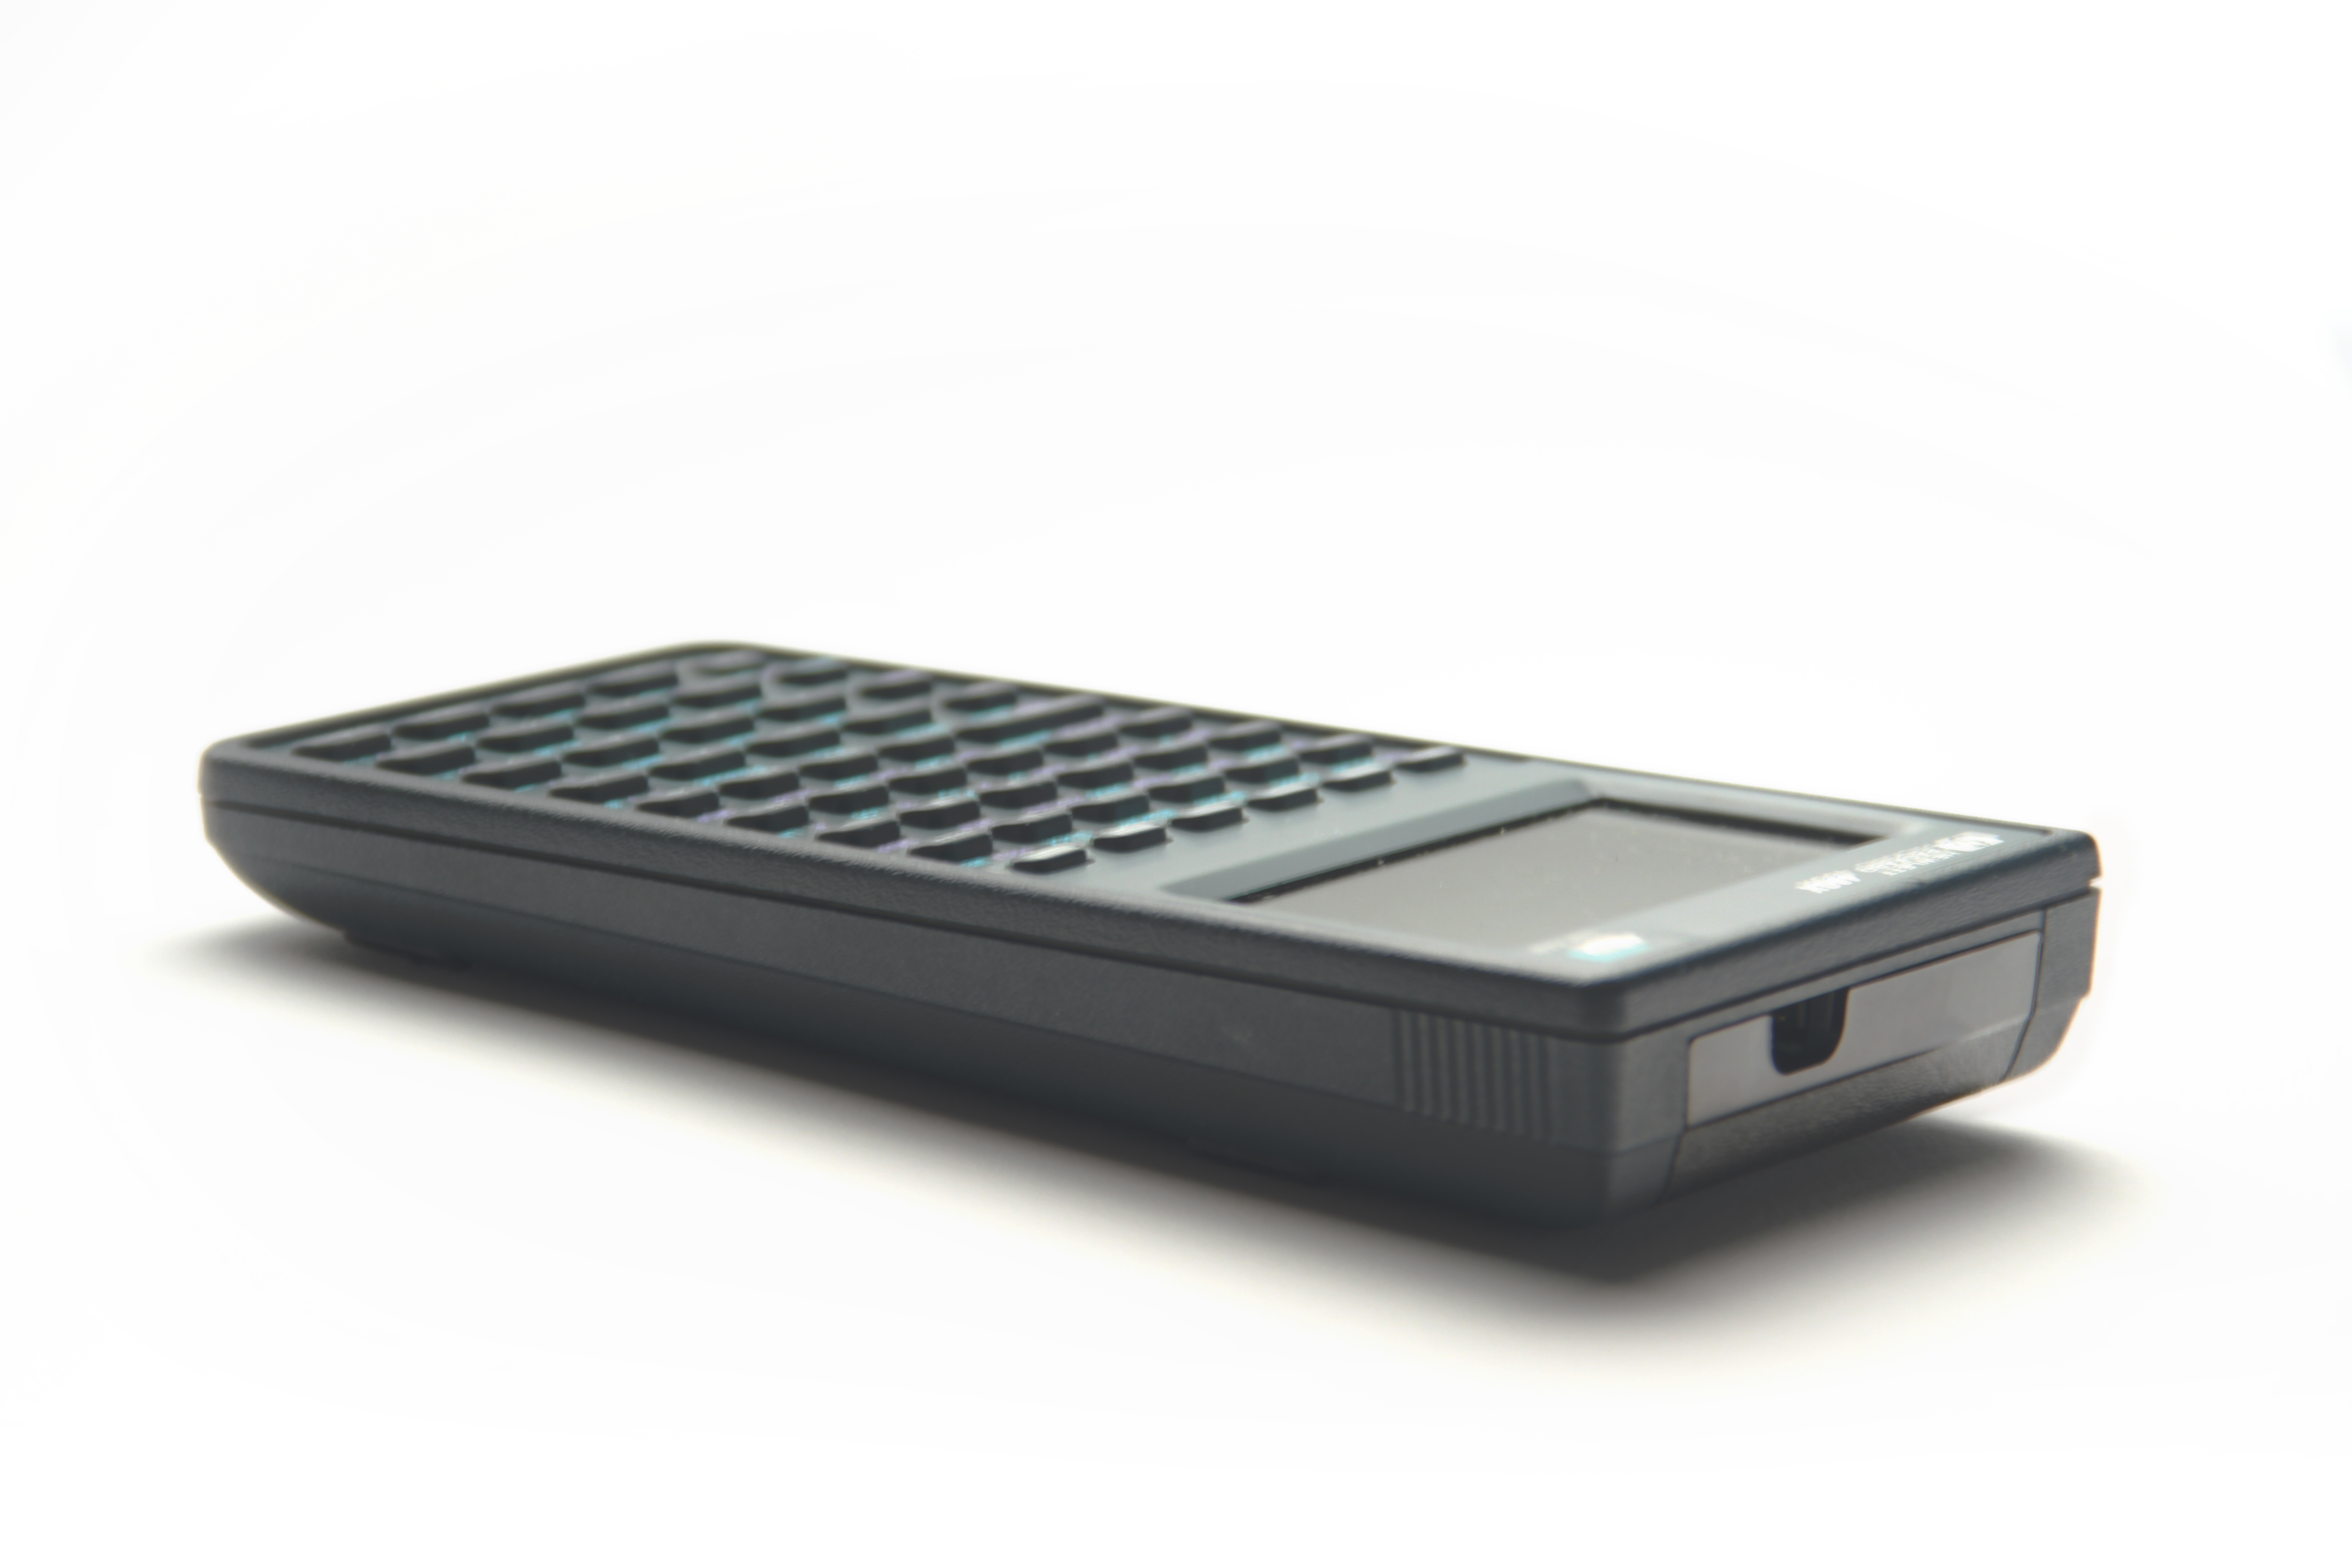
\includegraphics[width=0.4\linewidth]{hp}
    
    i també ha inspirat altres llenguatges com \emph{Factor, PostScript o REBOL}
\end{frame}

\end{document}